%
% teil1.tex -- Beispiel-File für das Paper
%
% (c) 2020 Prof Dr Andreas Müller, Hochschule Rapperswil
%
% !TEX root = ../../buch.tex
% !TEX encoding = UTF-8
%
\section{Stochastische Differenzialgleichungen\label{brown:SDGL}}
\rhead{Stochastische DGL}

Ist eine gewöhnliche Differenzialgleichung (DGL) gegeben, kann das Verhalten eines Systems unter Berücksichtigung der Anfangsbedingungen vorhergesagt werden. Vom Anfangswert aus entwickelt sich die Funktion gemäss der Startbedingung und dem durch die DGL gegebenen Vektorfeld. %Für einen bestimmten Startwert und wert der Laufvariabel, kann ein bestimmter Funktionswert ermittelt werden.

In vielen Bereichen entspricht ein solch deterministisches System  nicht der Realität und suggeriert eine Aussagekraft, welche sich nicht mit Beobachtungen deckt und somit einen eher Geringen Wert hat. Es gibt viele Systemen, welche stark auf kleine Störeinflüsse reagieren. Dies führt dazu, dass sich die Lösung einer DGL gegenüber der Realität, zum Beispiel durch Rauschen, nicht perfekt deckt oder das Resultat sogar komplett divergiert.

Ein gutes Beispiel dafür ist folgendes System:
\begin{equation}
	\frac{dx}{dt} = - y
	\frac{dy}{dt} = x^2 + y
	\label{divergentEquation}
\end{equation}

In der Abbildung~\ref{divergentAndConvergentSystem} sind zwei unterschiedliche Trajektorien im Vektorfeld eingezeichnet, welches durch die Gleichung~\ref{divergentEquation} gegeben ist. In rot ist der Verlauf im Intervall  t = [0,3] mit dem Startwert (-1.7, -1.4) gegeben und in grün mit dem Startwert (-1.8, -1.4).

\begin{figure}
	\centering
	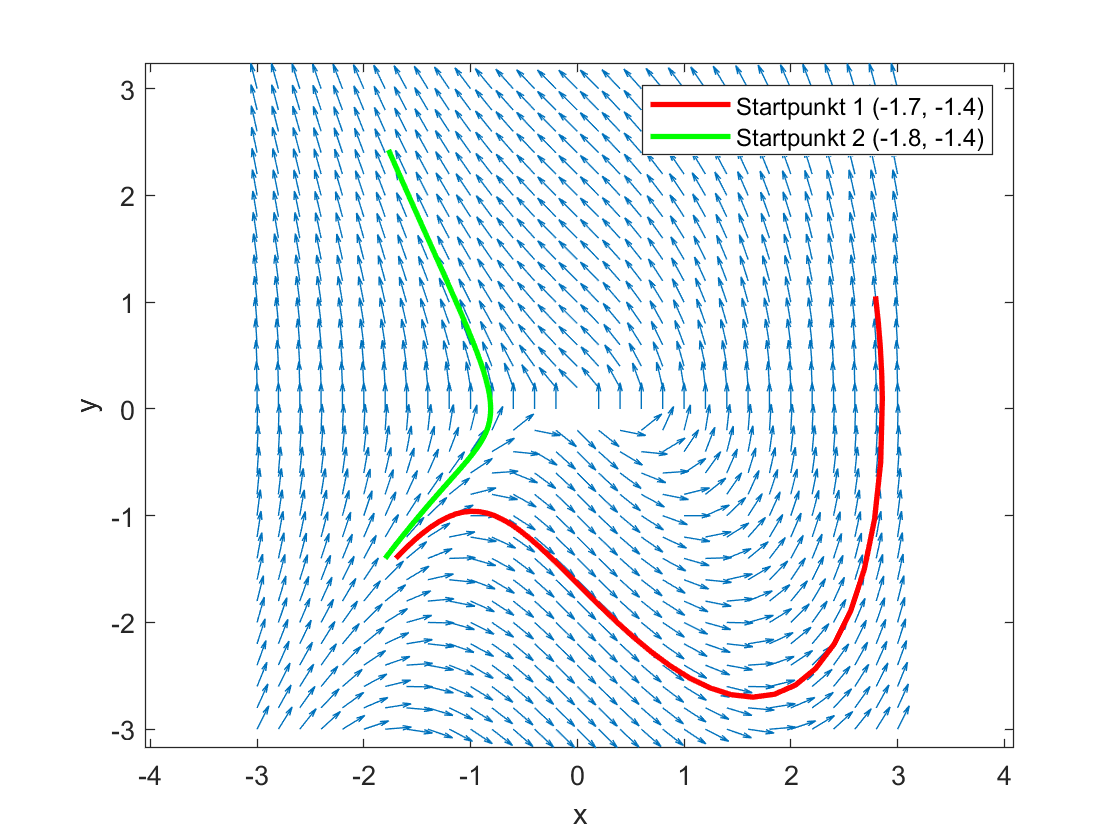
\includegraphics[width=0.8\textwidth]{papers/brown/images/Vektorfeld-mit-zwei-Pfaden.png}
	\caption{Zwei Pfade mit fast gleichem Startpunkt}
	\label{divergentAndConvergentSystem}
\end{figure}

Dieses System veranschaulicht schön, wie sich eine kleine Variation der Startbedingung auf den System-Verlauf auswirken kann. In diesem speziellen Fall konvergieren die Lösung mit grösserem $t$ wieder. Bedenkt man nun, dass eine solch kleine Variation durch stochastisches Rauschen erzeugt werden könnte, scheint es unsinnig eine fixe Lösung für ein solches System anzugeben - zumindest nicht ohne auf die Aussagekraft der Lösung hinzuweisen oder sogar den Lösungsraum genauer zu spezifizieren.

%In diesem System konvergieren alle Trajektorien zum Ursprung, ausser diese, welche Ihren Startwert exakt auf der Geraden $ y = x $ haben. Also kann ein kleiner Störeinfluss darüber entscheiden ob, der Wert zum gegen (0,0) konvergiert oder nach Unendlich divergiert. Wobei bei diesem Beispiel gesagt werden muss, dass in Realität der Startwert nie exakt auf die Gerade $ y = x $ fallen würde.

Um diesem Umstand gerecht zu werden, kann man die Möglichkeit von zufälligen Störungen beim Aufstellen eines Modells miteinbeziehen (in diesem Fall \textit{white noise}). Anstatt eine fixe Lösung zum Zeitpunkt $ t $ anzugeben, kann man eine Wahrscheinlichkeitsverteilung über die verschiedenen möglichen Endzustände definieren - et. voilà, man hat den Lösungsraum einer stochastische Differenzialgleichung (SDGL).

Formal kann eine stochastische DGL folgendermaßen notiert werden, 

\begin{equation}
\label{brown:SDGL:whiteNoise}
\dot{X}(t) = b(X(t)) + B(X(t))\xi(t) \quad (t>0)
\end{equation}

wobei $ B $ eine $ n $ x $ m $ Matrize mit Faktoren ist, welche beschreiben, wie sich Störungen auf die unterschiedlichen inneren Zustände des Systems auswirken. $ m $ ist demzufolge die Dimension der Störfunktion. In diesem Fall ist die Störung durch sogenanntes $ m $ dimensionales \textit{white noise} $ \xi(t) $ modelliert.

$ b $ ist der Driftvektor und beschreibt die erwartete Veränderung für jede Dimension des Systems. $ B $ ist die Dispersionsmatrix und beschreibt wies ich das $m$-dimensionale Rauschen aud das $n$-dimensionale System auswirkt. Dabei beschreibt die Diagonale der Matrix wie stark sich das Rauschen auf jede Dimension auswirkt und die Dreieckberreiche der Matrix beschreiben die Beeinflussung der Dimensionen untereinander. Alles in allem beschreiben $ b $ und $ B $ die Dynamik des Systems. 

\begin{align*}
		b = 
	\begin{pmatrix}
		b_{1} \\
		...\\
		b_{m}\\ 
	\end{pmatrix}
	, \quad
	B = 
	\begin{pmatrix}
		B_{11} & ... & B_{1m} \\
		& ... & \\
		B_{n1} & ... & B_{nm} 
	\end{pmatrix}
\end{align*}


Für die Modellierung von stochastischem Verhalten, ist der Wiener Prozess $ W(t) $ ein zentrales Konzept, zumal \textit{White noise} $ \xi(t) $ als die Ableitung vom Wienerprozess $ \frac{dW(t)}{dt} $ modelliert werden kann. Somit kann die SDGL aus \ref{brown:SDGL:whiteNoise} folgendermaßen geschrieben werden:

\begin{equation}
	\frac{dX(t)}{dt} = b(X(t)) + B(X(t)) \frac{dW(t)}{dt} \quad (t>0)
\end{equation}

Nun sollte man mit $ dt $  multiplizieren, weil die Gleichung sonst nicht sinnvoll ist, denn $ \frac{dW(t)}{dt} $ ist nicht klar differenzierbar. Dies ist den Eigenschaften des Wienerprozesses geschuldet. Gemäß der Definition ändert sich die Zufalls variable in jedem Schritt dem Erwartungswert und der Varianz entsprechend, ohne dabei von vorhergehenden Werten abzuhängen. Dieses unstetige verhalten ist nicht auf Grund (nicht definierter) Änderungsraten nicht differenzierbar.
! Überarbeiten, nicht differenzierbar? ?erweitern? ! 

Bei SDGLs wird das $ dt $ im Nenner oft mit $ dt $ multipliziert, um die Gleichung in die sogenannte \glqq{}Ito-Form\glqq{} zu bringen.

\begin{equation}
	dX(t) = b(X(t)) dt + B(X(t)) dW(t)
\end{equation}

%In dieser Form erkennt man auch besser, dass die SDGL aus zwei Teilen besteht. Der Term $ b((X(t)) $ ist der \glqq{}Drift\glqq{}-Term, der den deterministischen Teil der Bewegung darstellt, während $ B((X(t)) $ der \glqq{}Diffusions- oder Volatilitäts-Term\glqq{} ist, der den stochastischen Teil der Bewegung darstellt.

% So kommt man auf die ITO-sche Kettenregel????

Man kann dem Wiener Prozess auch fraktale Eigenschaften zusprechen, da man den Ausschnitt des zufällig beeinflussten Prozesses beliebig gross oder klein wählen kann und die keinen Einfluss auf die Eigenschaften des beobachteten Verhalten hat.


\subsection{Simulation mittels der Euler-Maruyama-Methode
\label{brown:Simulation}}
\rhead{Simulation} %Kurz-Titel der Section

Die Brownsche Bewegung kann relativ einfach simuliert werden mittels der Eueler-Maruyama-Methode.

Diese nummerische Methode wird oft zur Simulation von stochastischen Differentialgleichungen (SDGLs) verwendet und basiert auf der bekannten Euler-Methode zur Lösung von gewöhnlichen Differentialgleichungen. Die Idee ist, die SDGL in diskrete Zeitschritte zu zerlegen und den deterministischen und stochastischen Anteil separat zu behandeln. Die Methode hat zwar gewisse Einschränkungen hinsichtlich ihrer Genauigkeit und Stabilität, ist aber dennoch mitunter auf Grund ihrer Einfachheit weit verbreitet.

%SDEs sind Differenzialgleichungen, welche den Einfluss von zufälligen Prozessen, wie zum Beispiel Rauschen, auf ein dynamisches System berücksichtigen können. Sie bestehen aus einem deterministischen Anteil, der die zugrundeliegende Dynamik beschreibt, und einem stochastischen Anteil, der einen zufälligen Einfluss in Betracht zieht. 

Gegeben sei eine SDGL der folgenden Form:
\begin{equation}
	\mathrm{d}X(t) = a(X(t), t) \mathrm{d}t + b(X(t), t) \mathrm{d}W(t),
\end{equation}
wobei $ a(X(t), t) $ den deterministische Anteil darstellt, $ b(X(t), t) $ der stochastische Anteil ist und $ W(t) $ ein Wiener-Prozess ist, der das Rauschen repräsentiert. Die Methode beginnt mit einer Anfangsbedingung $X(0) = X_0$.

Um die SDGL mittels der Euler-Maruyama-Methode zu simulieren, geht man wie folgt vor:

\begin{enumerate}
	\item Man wählt eine Schrittweite $\Delta t > 0$ und teilt das Zeitintervall $[0, T]$ in $N$ gleich große Teilintervalle der Länge $\Delta t$: $t_0 = 0, t_1 = \Delta t, \dots, t_i = i\Delta t, \dots, t_N = T$.
	\item Für jeden Zeitschritt $i$ von $0$ bis $N-1$ werden die Werte der Funktion $X(t)$ an den diskreten Zeitpunkten $t_i$ berechnet,
	\begin{equation}
		X(t_{i+1}) = X(t_i) + a(X(t_i), t_i) \Delta t + b(X(t_i), t_i) \sqrt{\Delta t} \cdot Z_i,
	\end{equation}
	wobei $Z_i$ unabhängige standardnormalverteilte Zufallsvariablen sind.
	\item Diese Berechnungen führt man iterativ für alle Zeitschritte durch.
\end{enumerate}

\begin{equation}
	X_{n+1} = X_n + f(X_n,t_n) \Delta t + g(X_n,t_n) \Delta W_n
\end{equation}

Diese Funktion $ f(X_n,t_n) $ beschreibt dabei den deterministischen Teil der SDGL, im Kontext der Brown'schen Bewegung kann man es auch "drift nennen", welcher nicht nur von zufälligen Einflüssen bestimmt ist. Man muss jedoch erwähnen, dass er Erwartungswert zu jedem Zeitpunkt dem Startwert entspricht, also der zu erwartende Dritt 0 ist. 


Dies ist auch der Teil, der durch eine harmonische Analyse untersucht werden kann. Das Rauschen ("white noise"), welches hier mit $ g(X_n,t_n) $ beschrieben ist, enthält keine Information und kann somit nicht analysiert werden. $ \Delta W $ beschreibt die Geschwindigkeit, mit welcher der stochastische Prozess ablaufen soll und $ W_n $  beschreibt den Wiener Prozess oder die Brownische Bewegung als Ganzes.

\begin{figure}
	\centering
	\begin{minipage}{0.45\textwidth}
		\centering
		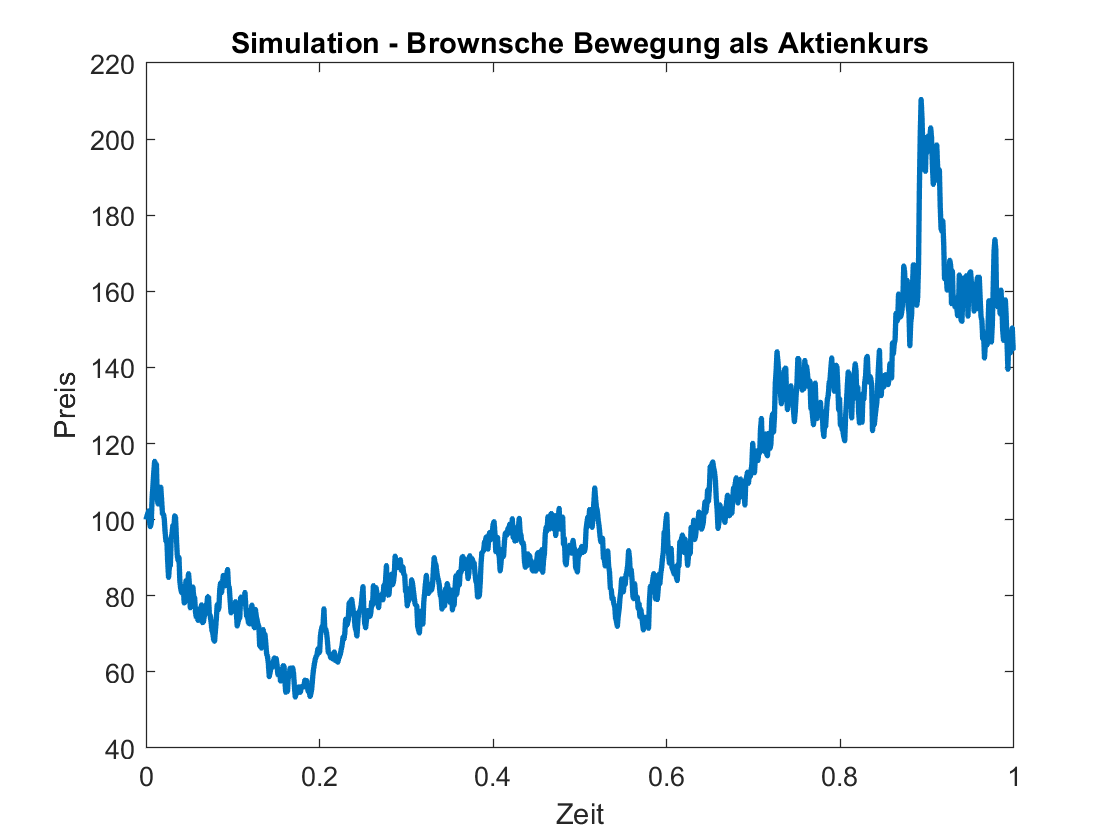
\includegraphics[width=\linewidth]{papers/brown/images/Aktienkurs-als-Brownische-Bewegung_2.png}
		\caption{1D Brownische Bewegung als Aktienkurs}
	\end{minipage}
	\hspace{0.05\linewidth}
	\begin{minipage}{0.45\textwidth}
		\centering
		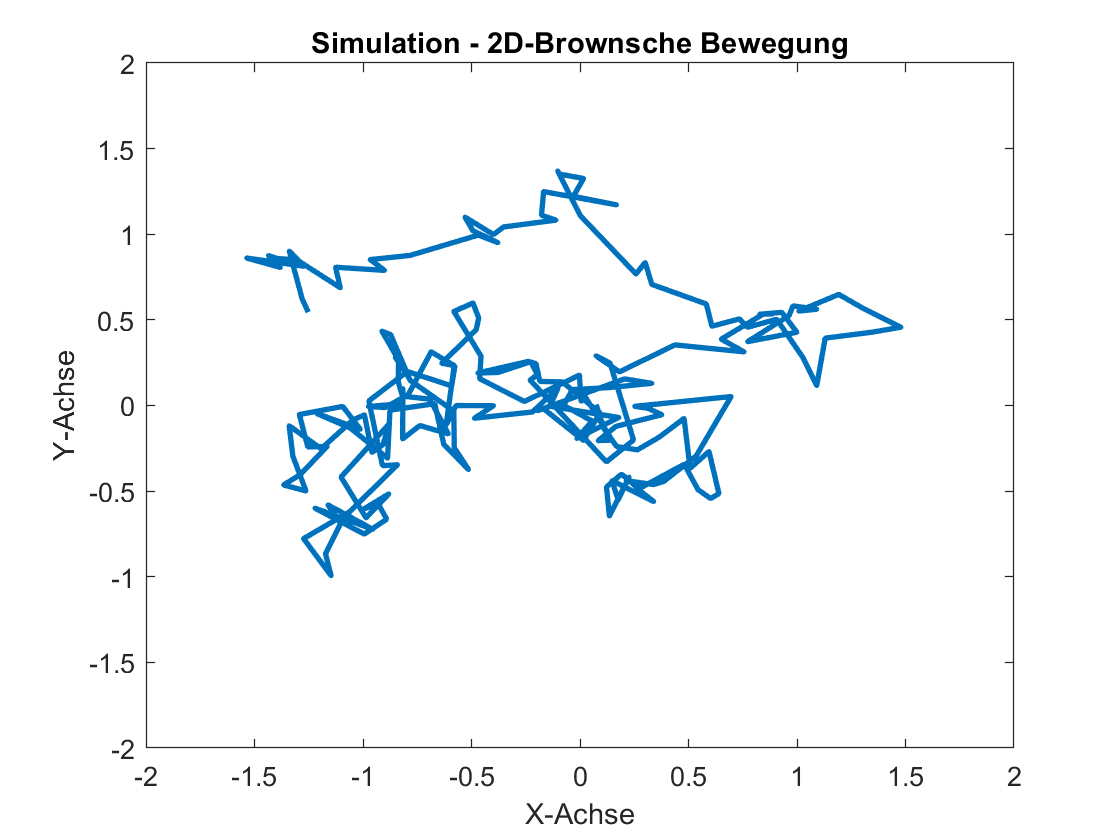
\includegraphics[width=\linewidth]{papers/brown/images/Brownische-Bewegung-Simuliert_2.png}
		\caption{Simulation einer Brownischen Bewegung in 2D}
	\end{minipage}
	\label{2D3Dbrownian}
\end{figure}

In der Abbildung ... ist wurde diese Simulations-Methode in einer Dimension angewandt. Man kann vielleicht schon erahnen, dass die zugrundeliegende Mathematik auf Börsenkurse anwendbar sein könnte. Führt man die Simulation für zwei Achsen durch und verbindet die einzelnen Simulationsschritte mit Linien, ergibt sich das Bild einer typischen Brownischen Bewegung.


\subsection{ITO
\label{brown:ito}}
\rhead{Ito} %Kurz-Titel der Section
Itō Kiyoshi war ein japanischer Mathematiker, der seine Kariere der Stochastik widmete und heute als Begründer der stochastischen Analysis zählt. So legte er auch einen Grossteil des Fundaments auf dem stochastische Differenzialgleichungen beruhen. 

Nach ihm ist auch die Itō'sche Form einer SDGL benannt, bei welcher die Gleichung mit dem Nenner des Differenzialquotienten multipliziert wird. Diese Form ist Ausgangslage viele seiner "Konzepte?", bietet jedoch auch den Vorteil, dass keine Differenzierbarkeit suggeriert wird. Denn ein stochastische Prozess kann nicht ohne weiteres abgeleitet werden.

Ein wichtiges Werkzeug, um mit stochastischen DIfferenzialgleichungen umzugenhen ist das Äquivalent zur Kettenregel, dem sogenannten Lemma von Ito. %Dieses wird auch im Abschnitt XXXX für das Black-Scholes-Merton Modell verwendet. Auch nach ihm benannt ist die "ito-Form", in welcher die Gleichungen notiert sind XXX.%

Hier ein Beispiel einer stochastischen Differentialgleichung (SDG) für einen Prozess X(t) in Ito-Form:
\begin{equation}
	dX = a(X,t) dt + b(X,t) dW
\end{equation}

Angenommen, wir haben eine Funktion f(X,t), wobei X eine Lösung der obigen SDG ist. Dann kann die Änderung von f in Bezug auf X und t wie folgt geschrieben werden:

Die Funktion f(X,t) und das Ito-Lemma:
\begin{equation}
	df = \frac{\partial f}{\partial t} dt + \frac{\partial f}{\partial X} dX + \frac{1}{2} \frac{\partial^2 f}{\partial X^2} (dX)^2	
\end{equation}

%Dabei sind ∂f/∂t und ∂f/∂X die partiellen Ableitungen von f nach t und X, und ∂²f/∂X² ist die zweite partielle Ableitung von f nach X. Der Term (dX)² ist im Ito-Kalkül durch (b^2 dt) ersetzt, was auf die Eigenschaften der Brown'schen Bewegung (oder Wiener-Prozess) zurückzuführen ist.

Dieses Lemma erlaubt es uns, Differentialgleichungen für Funktionen von stochastischen Prozessen abzuleiten, was bei der Lösung von SDGs hilfreich ist.


Das Einsetzen der SDG in das Ito-Lemma ergibt:
\begin{equation}
	df = \frac{\partial f}{\partial t} dt + \frac{\partial f}{\partial X} (a dt + b dW) + \frac{1}{2} \frac{\partial^2 f}{\partial X^2} (b^2 dt)
\end{equation}

Die Funktion $ a(X,t) $ ist der "Drift"-Term, der den deterministischen Teil der Bewegung darstellt, während $ b(X,t) $ der "Diffusions-" oder "Volatilitäts-Term" ist, der den stochastischen Teil der Bewegung darstellt.

%Ein wichtiger Aspekt des Ito-Kalküls ist die Ito'sche Lemma, eine Erweiterung der Kettenregel aus der gewöhnlichen Differentialrechnung für Funktionen von stochastischen Prozessen. Die genaue Form des Ito'schen Lemmas kann komplex sein, aber in einer einfacheren Form lautet es wie folgt:


%Gemäss Itō ist das Integral einer gewöhnlichen SDGL folgendermassen definiert:
%Weglassen?



